% コンパイル方法: lualatex filename.tex
\RequirePackage{plautopatch}

\documentclass[a4paper, 10pt]{ltjsarticle}


% マージン設定
\usepackage[top=20mm, bottom=20mm, left=20mm, right=20mm]{geometry}

% LuaLaTeX用日本語対応パッケージ
\usepackage{luatexja}
\usepackage{luatexja-fontspec}

% 必要なパッケージ
\usepackage{fontspec}
\usepackage{titlesec}
\usepackage{graphicx}
\usepackage{amsmath}
\usepackage{amssymb}
\usepackage{hyperref}
\usepackage[english, japanese]{babel}
\usepackage{multicol} % 二段組用パッケージ
\usepackage{indentfirst}
\usepackage{tikz} % カスタム点線用
\usepackage{authblk} % 著者・所属パッケージ
\usepackage{here}
\usepackage{caption}
\usepackage{tabularx}
\usepackage{subcaption}

% \setmainfont[Ligatures=TeX]{Times New Roman}
% \setmainjfont[BoldFont=MS Gothic]{MS Mincho}

\renewcommand{\baselinestretch}{0.94}

% セクション見出しのカスタマイズ
\titleformat{\section}
  {\fontsize{10pt}{10pt}}
  {\thesection.}
  {1em}{}

\titleformat{\subsection}
  {\fontsize{10pt}{10pt}}
  {\thesubsection}
  {1em}{}

\titleformat{\subsubsection}
  {\fontsize{10pt}{10pt}}
  {\thesubsubsection}
  {1em}{}

  \setlength{\parindent}{1em}

\captionsetup[table]{skip=0pt}
\captionsetup[subfigure]{font=normalsize}
\setlength{\belowcaptionskip}{0.5em} % キャプション下の余白を設定


\titlespacing*{\section}{0em}{1em}{0em}
\titlespacing*{\subsection}{0em}{1em}{0em}

\pagestyle{empty}


\begin{document}

\setlength{\abovedisplayskip}{-0.5em}
\setlength{\belowdisplayskip}{0.5em}
% \setlength{\columnsep}{7.5mm}

\twocolumn[
    \begin{center}
        {\vspace{-1em}}

        {\fontsize{15pt}{15pt}\selectfont{クロスレイヤシミュレータにおける無線LAN評価モデルの検討}}

        {\vspace{1.3em}}

        {\fontsize{13pt}{13pt}\selectfont{A Study of a Wireless LAN Evaluation Model in a Cross-Layer Simulator}}
    \end{center}

    \vspace{0.1em}

    \begin{flushright}
      {\fontsize{11pt}{11pt}\selectfont{T5-16 \, 下沢亮太郎}}
      \\
      {\fontsize{11pt}{11pt}\selectfont{指導教員 \, 設樂勇}}
    \end{flushright}

    \vspace{1em}

    \thispagestyle{empty}
]

\section{はじめに}
% 近年,無線通信端末利用者の急増に伴い様々な場所で無線通信システムが利用されており,今後も利用の増加と発展が見込まれている.近年の無線通信技術の進歩に伴い,システムが高機能化・複雑化しており,従来のようにレイヤごとに独立した性能評価を行う手法では通信全体の実用的な評価を十分に行うことが困難になりつつある.そのため,通信全体をクロスレイヤで評価できる計算機シミュレータの開発が求められている.本研究ではクロスレイヤシミュレータにおけるMACレイヤの挙動をシミュレートする機能の開発を行い,その有効性を評価することを目指した.
% 従来のように,各レイヤを独立して評価する手法では,通信全体を俯瞰した実用的な性能評価が難しくなりつつある.そのため,物理層から上位層までを跨いで統合的に評価できるクロスレイヤシミュレータの開発が求められている.
% 本研究では,クロスレイヤシミュレータの一部としてMAC(Medium Access Control)レイヤの挙動をシミュレートする機能を開発し,その有効性を評価することを目的とする.
% しかし,各レイヤごとに性能のボトルネックが存在するため,他レイヤとの統合した評価が必要不可欠である.
% 本研究では,IEEE 802.11規格に基づくCSMA/CA(Carrier Sense Multiple Access with Collision Avoidance)方式を用いたMAC(Medium Access Control)レイヤの挙動を再現したモデルを構築し,クロスレイヤシミュレータの一部として動作を再現するシミュレータを開発した.その上で,開発したシミュレータの動作が理論値と一致することを評価し,その有効性を検証することを目指す.


近年,無線通信端末の利用者が急増し,多様な場所で無線通信システムが活用されており今後も利用の拡大と機能の高度化が見込まれる.一方で,無線通信技術の進歩に伴いシステム自体はますます高機能化・複雑化している.
しかし,研究開発の現場では各レイヤごとに検討が行われており,単一レイヤのみの評価では通信システム全体の性能を十分に把握することができない.
本研究では,無線通信全体の品質を総合的に評価するために,実環境の電波伝搬特性を考慮した物理層とMAC(Medium Access Control)層が連携したシミュレータの開発の一環として,IEEE 802.11規格に基づくCSMA/CA(Carrier Sense Multiple Access with Collision Avoidance)方式を用いたMAC層の動作に則った無線LAN(Local Area Network)モデルを開発し,その精度を評価することを目指す.


\section{無線LAN通信モデル}


\subsection{CSMA/CA方式}

IEEE 802.11規格では,CSMA/CAと呼ばれるアクセス制御方式を採用している.図\ref{CSMA/CA}にCSMA/CAの概要を示す.
CSMA/CAでは,送信したいフレームが発生した際,まずキャリアセンス(CS)を行い,チャネルが空いている(Idle)かどうかを確認する.
チャネルがIdleの場合は,各端末がバックオフ時間としてランダムなスロット数を生成し,その時間だけ待った後に再度キャリアセンスを行い,チャネルがIdleのであればフレームを送信し,使用中(Busy)だった場合はフレームを送信できるまでバックオフ時間を持ち越す.複数の端末が同じスロット数となった場合には送信タイミングが同時になり,衝突が発生するため再送制御が必要となる.

無線LANシステムでは2進数バックオフ方式を採用している.バックオフ制御に用いるContention Window(CW)は,最小値を15とし,最大値の上限を1023スロットとして衝突回数の増加に従いCWサイズは.再送回数を$n$とすると,CWサイズの最大値$\mathrm{CW}_{\max}$とスロット数$s$は


\begin{align}
  \mathrm{CW}_{\max} &= 2^{4 + n} - 1
\end{align}

\begin{align}
  s &= \mathrm{randint}(1, \, \min(c_{\max}, \, 1023))
  \label{slot}
\end{align}

で求められる.

衝突が発生するたびにCWサイズの最大値は2倍に増加するため,再送回数が増えるほどバックオフ時間が長くなることで他端末と同じCWサイズを生成することがなくなり,衝突確率を低減することができる.一方で,2進数バックオフ方式ではCWサイズの増加がオーバーヘッドを引き起こし,スループットの低下につながる.


% 本シミュレータでは,端末クラスにスロット生成メソッドを実装し,インスタンスごとにスロット数と再送回数$n$を保持することで,各端末が送信を試みる際の待機時間を動的に設定する処理を実装した.

本シミュレータでは,端末単位でスロット数と再送回数$n$を保持することで,各端末が送信を試みる際の待機時間を動的に設定する処理を実装した.


\begin{figure}[htbp]
  \centering

  \begin{subfigure}{\columnwidth}
    \centering
    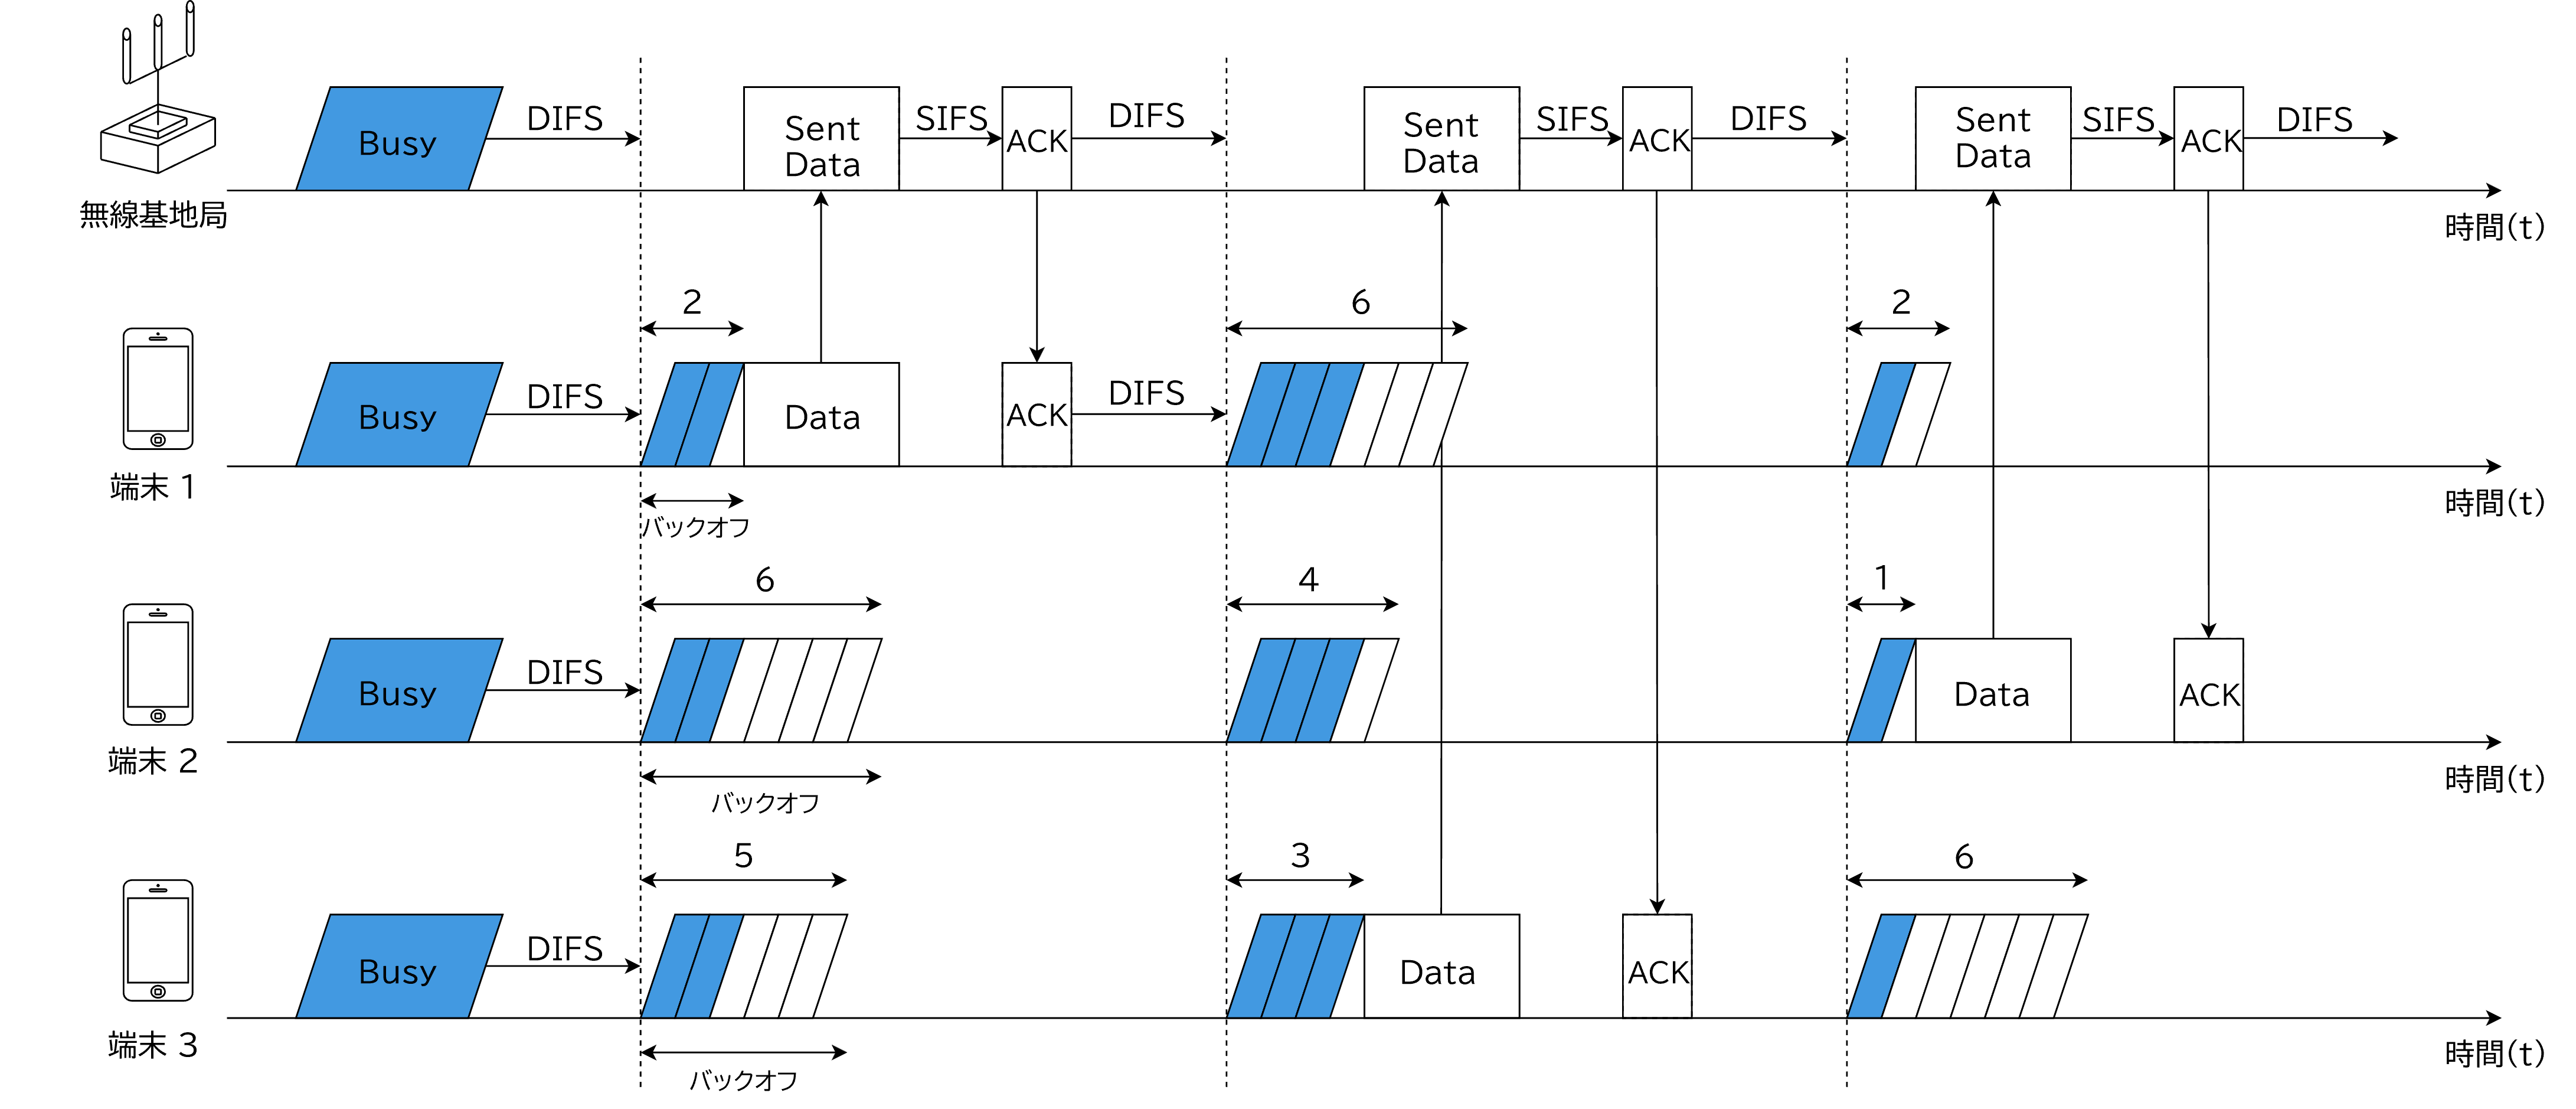
\includegraphics[width=1\columnwidth]{./assets/csma-ca-s.png}
    \caption{CSMA/CA成功時}
    \label{1a}
  \end{subfigure}


  \begin{subfigure}{\columnwidth}
    \centering
    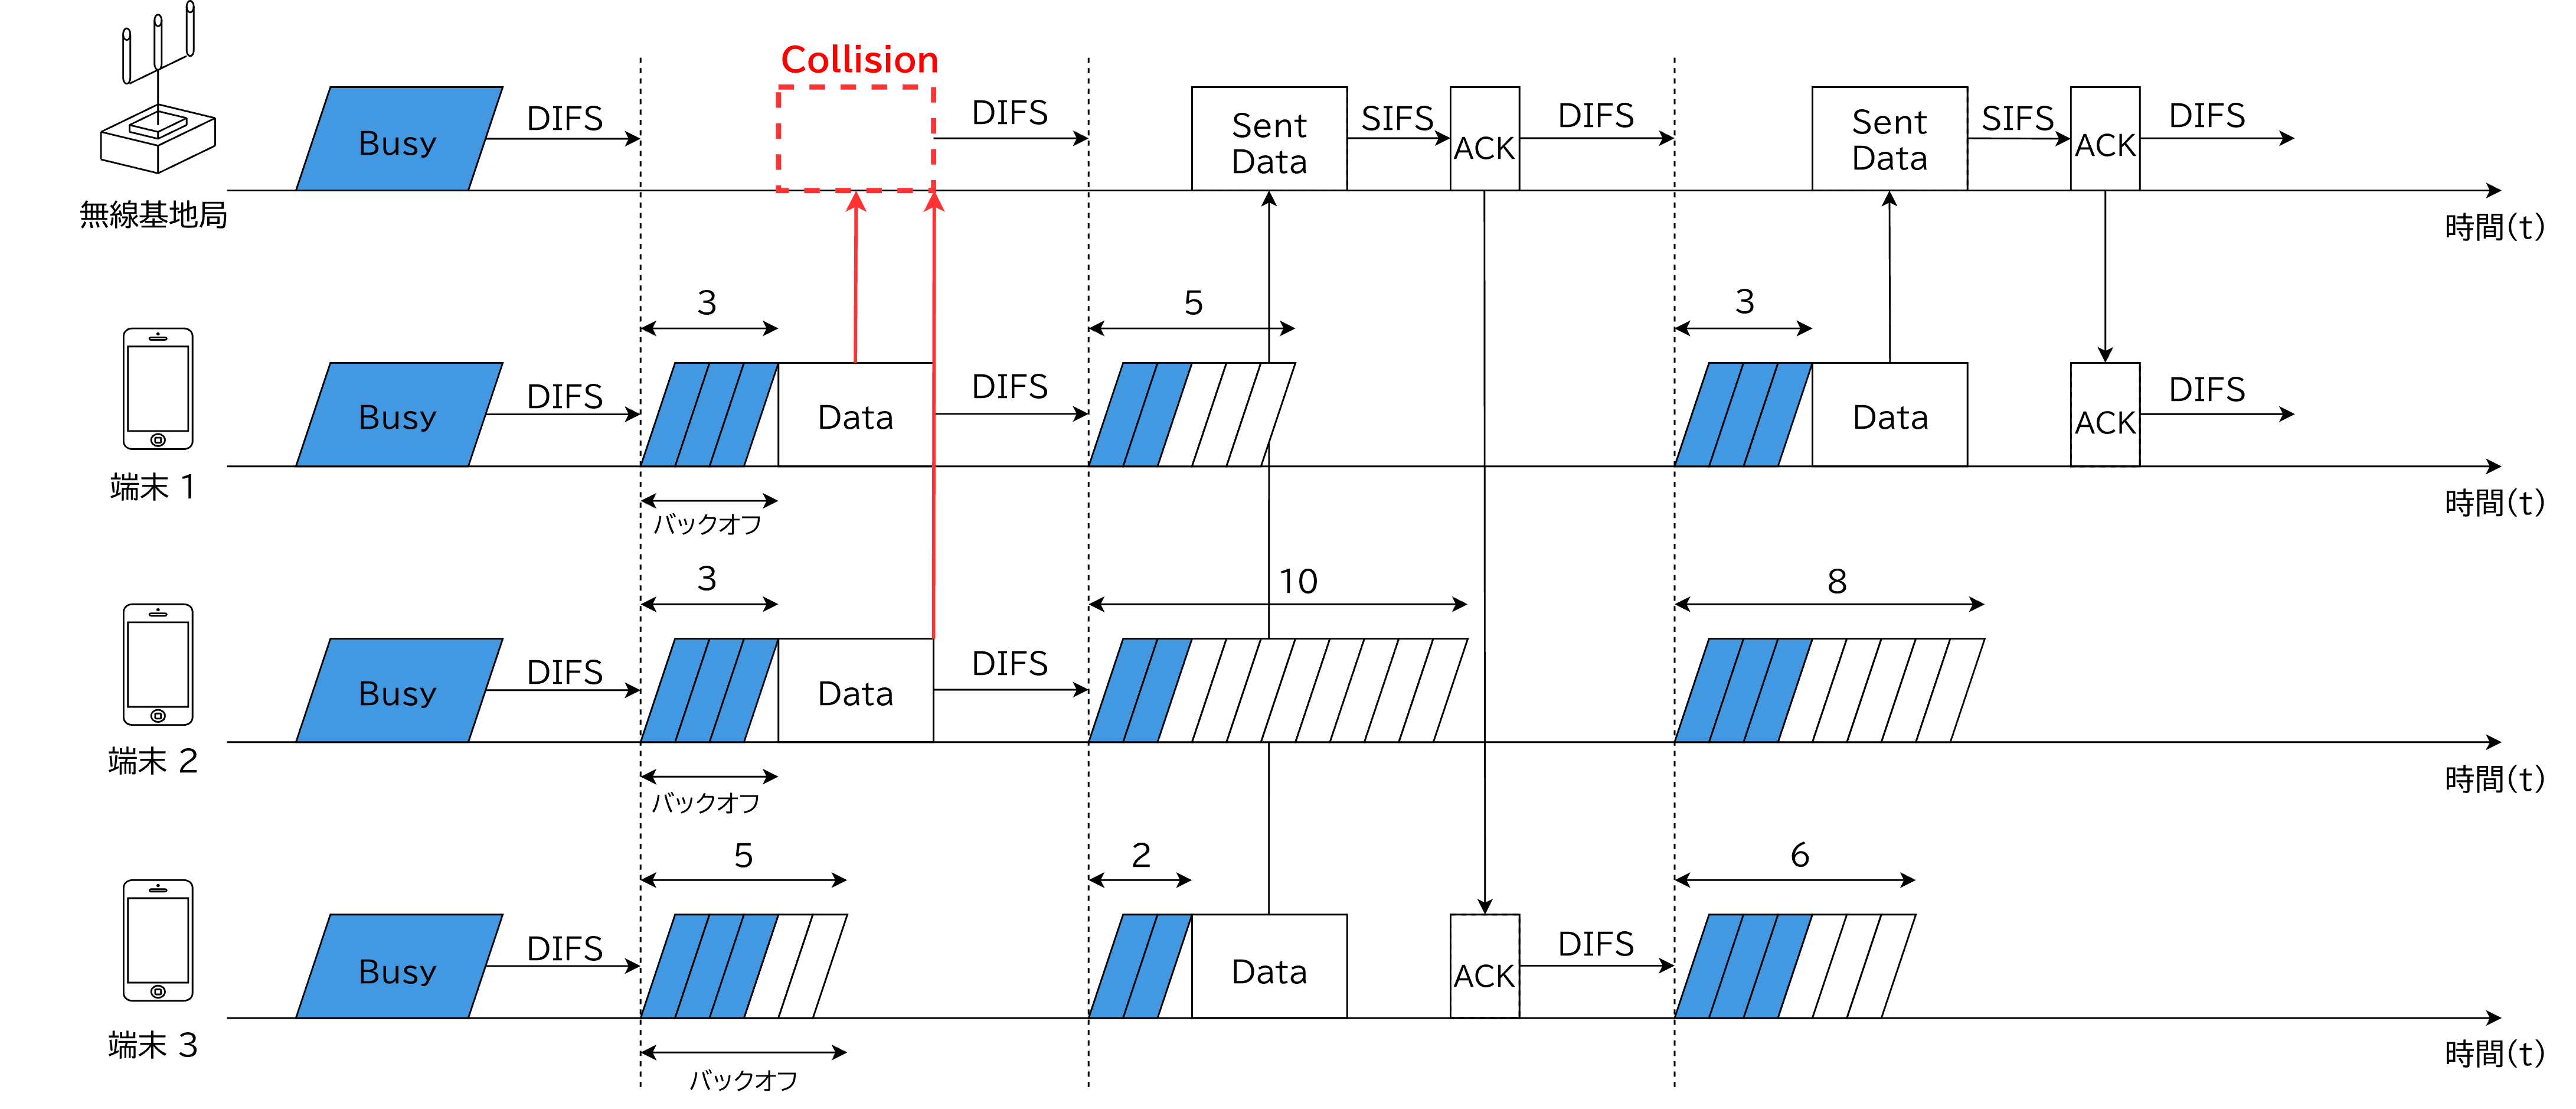
\includegraphics[width=1\columnwidth]{./assets/csma-ca-f.png}
    \caption{CSMA/CA衝突時}
    \label{1b}
  \end{subfigure}


  \caption{CSMA/CAの概要}
  \label{CSMA/CA}
\end{figure}

\vspace{-3em}

\subsubsection{IFSによる優先制御}

フレーム間にはIFS(Inter Frame Space)と呼ばれる待機時間が設定されている.IFSの長さは6種類存在し,代表的なものにDIFS(Distributed Inter Frame Space)とSIFS(Short Inter Frame Space)がある.これらは,フレームの優先順位に基づいてどのIFSを選択するかが決定される.

DIFSはデータフレーム送信時に適用されるIFSであり,端末は送信開始前にDIFS時間($34\mathrm{\mu s}$)待機してからデータフレームを送信する.
一方,ACK(ACKnowledgment)フレームのように失敗すると再送制御が必要となる優先度の高い制御フレームは,DIFS時間待つと他端末のデータフレームと競合する可能性があるため,より短いSIFS時間($16\mathrm{\mu s}$)を用いることで優先的に送信するように設定されている.




\subsection{フレーム構成モデル化}

本研究では,MAC層に着目した無線LAN通信の挙動を評価するため,UDP(User Datagram Protocol)レベルのフレーム構成をモデル化し,図\ref{packet}にその構成図を示す.

無線LANフレームにはPLCP(Physical Layer Convergence Protocol)プリアンブルやMACヘッダー,FCS(Frame Check Sequence)というオーバーヘッドに加え,ACKフレームの送信やCSMA/CA特有のDIFS・SIFSなどのフレーム間隔,バックオフ動作も含まれる.その他にもLLC(Logical Link Control)ヘッダやIPヘッダなどが含まれるが,シミュレーションの都合でモデル化した.

% 無線LAN通信では,データ送受信時にPLCP(Physical Layer Convergence Protocol)プリアンブルやMACヘッダ,FCS(Frame Check Sequence)などの制御情報のオーバーヘッドに加え,ACKフレームの送信やCSMA/CA特有のDIFS・SIFSなどのフレーム間隔,バックオフ動作も必要となる.

% することで,ACKフレームやCSMA/CA特有のフレーム間隔(DIFS, SIFS),バックオフなど,MAC層における主要な動作の評価を効率良く行えるようにした.

% 本研究では,UDP(User Datagram Protocol)レベルの無線LAN通信を再現するためにフレーム構成をモデル化した.図\ref{packet}にモデル化したフレームの構成図を示す.

% 無線LAN通信では,データ送受信時にPLCP(Physical Layer Convergence Protocol)プリアンブルやMACヘッダ,FCS(Frame Check Sequence)などの制御情報のオーバーヘッドに加え,ACKフレームの送信やCSMA/CA特有のDIFS・SIFSなどのフレーム間隔,バックオフ動作も必要となる.

% 本研究では,MAC層におけるCSMA/CA方式の挙動を中心に,UDP(User Datagram Protocol)レベルのデータ送受信を再現することを目的としてフレーム構成をモデル化した.

% 通常,無線LANのフレームには物理層におけるPLCP(Physical Layer Convergence Protocol)プリアンブルや,MACヘッダ,FCS(Frame Check Sequence)などの制御情報が付与されるほか,さらに上位層のLLC(Logical Link Control)ヘッダやIP(Internet Protocol)ヘッダなどが付加される.しかし本研究のシミュレーションでは,MAC層での衝突やバックオフ時間を中心に検討するため,これらの上位層ヘッダを含む詳細な要素を全て実装すると計算負荷が増大し実行時間が大きくなる恐れがある.

% そこで本シミュレータでは,図\ref{packet}に示すようにプリアンブルやMACヘッダ,FCSなど基本的な制御情報のみを考慮したフレームをモデル化し,LLCやIPなどシミュレーションの目的上必須でないヘッダについては省略している.また,ACK(ACKnowledgment)フレームの送信やCSMA/CA特有のDIFSおよびSIFSなどのフレーム間隔,バックオフ動作などは実際の無線LAN規格(IEEE 802.11)をもとに取り入れている.


% 本研究では,MAC層に着目した無線LAN通信の挙動を評価するため,UDPレベルのフレーム構成を簡略化してモデル化した.本来,無線LANフレームにはPLCP(Physical Layer Convergence Protocol)プリアンブルやMACヘッダ,FCS(Frame Check Sequence)に加え,LLC(Logical Link Control)ヘッダやIPヘッダなども含まれるが,シミュレーションの都合上省略してモデル化している.これにより,ACKフレームやCSMA/CA特有のフレーム間隔(DIFS, SIFS),バックオフなど,MAC層における主要な動作の評価を効率良く行えるようにした.

% このため,物理層のみを考慮したシミュレーションと比べ,実環境でのスループットは低下することから,クロスレイヤでの検討が必要である.

\begin{figure}[htbp]
  \centering
  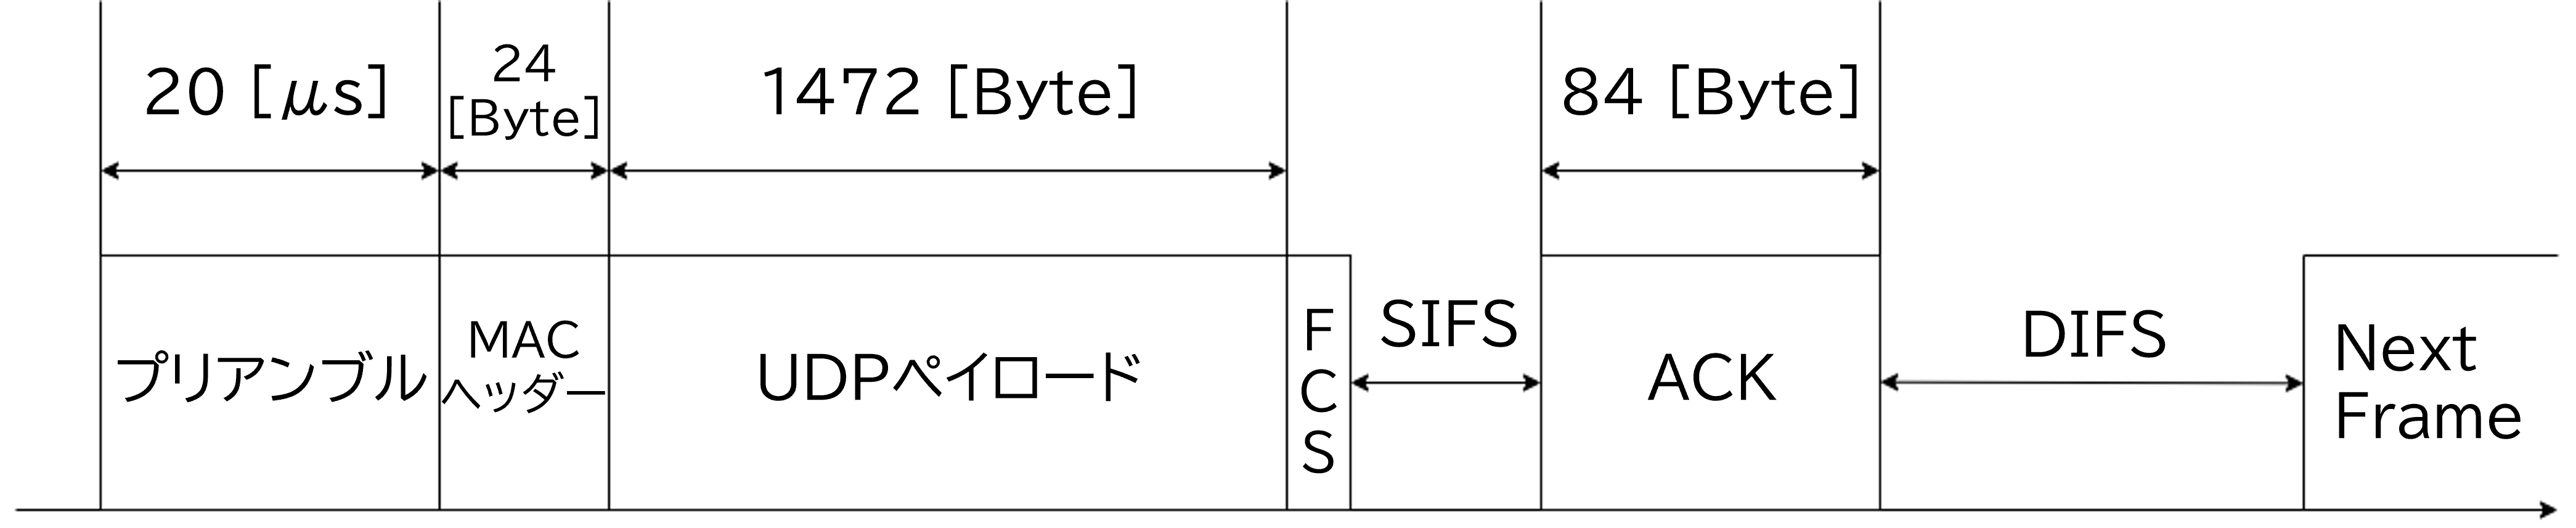
\includegraphics[width=1\columnwidth]{./assets/packet.png}
  \caption{フレーム構成図}
  \label{packet}
\end{figure}

\vspace{-2em}

\vspace{-0.5em}

\section{実装とシミュレーション設定}

本研究では,CSMA/CA方式を用いた無線LANを再現するために,Pythonを用いてシミュレータを作成した.シミュレータには,各端末を管理する端末クラスを導入し,端末ごとのCWサイズや再送回数の管理,バックオフ時間を決定するためのスロット数の管理,再送処理などの機能を実装している.

また,シミュレータ本体は標準ライブラリである\texttt{random}のみに依存するように設計した.これにより,バージョン差異による影響を受けにくい後方互換性のあるシミュレータを実現した.



\vspace{-0.5em}

\subsection{シミュレーション条件}
表\ref{tab:sim-param}に,本研究で用いシミュレーション条件を示す.
モードを選択することでそれぞれの無線LAN規格(IEEE 802.11a/b/g)に対応できるように設計した.


\vspace{-1em}


\begin{table}[htbp]
  \centering
  \caption{シミュレーション条件の例}
  \label{tab:sim-param}
  \begin{tabular}{c|@{\hspace{1.8em}}l}
    \hline
    パラメータ & 値・例 \\
    \hline
    シミュレーション時間 & 60 \, \,$\mathrm{s}$\, \\
    スロット時間 (802.11a) & \, 9 \, \,$\mathrm{\mu s}$\, \\
    DIFS (802.11a) & 34 \, \,$\mathrm{\mu s}$\, \\
    SIFS (802.11a) & 16 \, \,$\mathrm{\mu s}$\, \\
    伝送レート & 24 \, \,Mbps\, \\
    端末数 & 80 \, \,台\, \\
    \hline
  \end{tabular}
\end{table}

\vspace{-2em}

\section{評価}
横軸を端末数,縦軸をスループットとしたシミュレーション結果と理論値を図\ref{fig:simulation-result}に示す.



理論値との差が一番大きい端末数が80台の場合でも+2.75\%程度の誤差に収まっていることが確認できる.また,端末数が増加するにつれて理論値との差が徐々に拡大することに対しては,参考とした文献\cite{paper}とのIP(Internet Protocol)レベルとUDPレベルのプロトコル上の違いからくるペイロード長の差などモデル化方法の違いが影響していると考えられる.
以上の結果から,本研究で構築したCSMA/CAベースの無線LANモデルは,理論値に対して概ね一致し,最大でも誤差がおよそ3\%にとどまることが示された.

\begin{figure}[htbp]
  \centering
  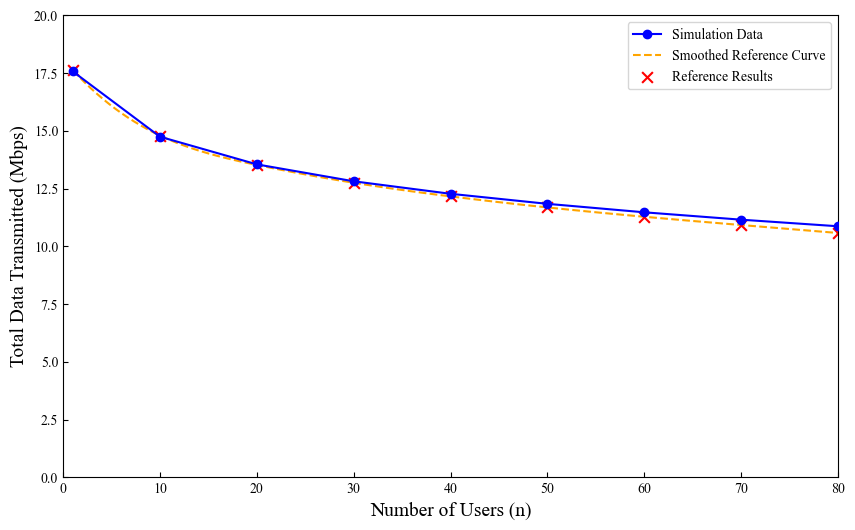
\includegraphics[width=1\columnwidth]{./assets/g3.png}
  \caption{シミュレーション結果}
  \label{fig:simulation-result}
\end{figure}

\vspace{-2em}

\section{まとめ}

本研究では,クロスレイヤシミュレータにおけるCSMA/CAを中心とした無線LANシステムのモデル化とそのシミュレータを開発し,精度を検証した.

今後の課題としては,連続送信ではなくポアソン分布などに従った送信間隔を導入し,より実際の通信頻度に近い状況を再現することが挙げられる.
さらに,端末ごとに伝送速度を変えられるようにすることや,各端末やアクセスポイントの位置情報を踏まえて受信時のSNR(Signal-Noise Ratio)を考慮し,衝突時でもフレームの複合が可能となるキャプチャ効果を導入することで,より実環境に近い通信環境を再現することが挙げられる.

\vspace{-0.5em}

\begin{thebibliography}{9}
  \bibitem{midori}守倉正博, 久保田周治, 『インプレス標準教科書シリーズ 改訂三版802.11 高速無線LAN教科書』, 株式会社インプレスコミュニケーションズ, 2016年
  \bibitem{paper}Y. Morino, T. Hiraguri, H. Yoshino, K. Nishimori, T. Matsuda, ``A Novel Collision Avoidance Scheme Using Optimized Contention Window in Dense Wireless LAN Environments*'' \, \textit{IEICE TRANS. COMMUN.}, VOL.E99-B, NO.11 NOVEMBER 2016
  \bibitem{11std}IEEE 802.11 Standard for Local and Metropolitan Area
  Networks, “Part 11: Wireless LAN Medium Access Control (MAC) and Physical Layer (PHY) Specifications,”  IEEE Std. 802.11, Mar. 2012.
  % \bibitem{book1}西森健太郎,平栗健史,『MIMOからMassive MIMOを用いた伝送技術とクロスレイヤ評価手法』, コロナ社, 2017年.
  % \bibitem{book2}設樂勇, 平栗健史, 谷口諒太郎, 西森健太郎, 『レイトレースを用いた3次元クロスレイヤシミュレータの開発』, 社団法人 電子情報通信学会 信学技報
\end{thebibliography}



\end{document}
